\chapter{Analisi statica}
Il primo passo di questo processo di analisi riguarda in primo luogo un approccio di tipo statico.

Questo tipo di analisi è usato per fare una prima esaminazione senza eseguirli su un sistema.
Per arrivare a tali risultati, si ispeziona il codice del file del malware, alla ricerca di varie caratteristiche, in base a quale strumento stiamo usando e al suo scopo.
Possiamo andare alla ricerca, più o meno approfondita, di chiamate di sistema particolari, indizi di offuscamento o crittografia anche tramite un'analisi dell'entropia di alcune sezioni del file, nonché più direttamente degli IoC già noti.
Si possono usare numerose tecniche, tra cui:

\begin{itemize}
    \item \textbf{Disassemblaggio o decompilazione} al fine di andare ad esaminare il codice più o meno ad alto livello del sorgente originale dell'eseguibile, anche se spesso questa pratica resta difficoltosa per tutte le ragioni dietro la reverse-engineering, con particolare attenzione degli autori del malware di rendere tecniche come questa il più difficili possibile
    \item \textbf{Analisi delle stringhe} per identificare IoC particolari come URL noti, indirizzi IP, o anche semplicemente nomi di chiavi di registro o file che normalmente non dovrebbe andare a toccare in un normale funzionamento
    \item \textbf{Estrazione dei payload} integrati all'interno del file, come exploit nascosti / crittografati o anche lo stesso codice del vero eseguibile, come nel caso dei file pacchettizzati, che tratteremo nelle successive sezioni
\end{itemize}

Infine, non necessariamente si deve trattare di un eseguibile: può anche essere analizzato un documento Office o un file PDF, anch'essi noti per essere potenziali vettori di attacco, includendo delle macro o del codice eseguibile al proprio interno.

\section{Struttura binari}
\label{chap:static_analysis_binary_structure}
Prima di andare nel dettaglio di quali tecniche sono state adottate per avere un sistema di analisi statica quanto più completo possibile, bisogna andare a illustrare sommariamente la struttura di un file binario.

Innanzitutto, un file eseguibile contiene sia codice che dati, ed è diviso in \textbf{sezioni}, che possono avere diversi permessi di lettura (read-only) o scrittura (read-write).
Questo è un dettaglio più importante di quanto ci aspetteremmo perché ad esempio un eseguibile potrebbe compiere tecniche di modifica della propria sezione di codice, impostandola come read-write, potendo eludere così in maniera piuttosto significativa tecniche di analisi statica, poiché il vero codice del software sarà creato durante la sua stessa esecuzione, e nella fase statica (come dice il nome stesso) non andiamo a lanciare alcun programma.

Un'altra area comune e rilevante è la \textbf{symbol table}, o "tabella dei simboli".
Questa contiene riferimenti a funzioni o variabili poste in altri file o librerie esterne, che nella prima fase di \emph{Assembling} sono stati trasformati in degli \emph{object file} distinti,
e come tali sono rilocabili, ossia non dipendono già da particolari indirizzi in memoria.
Quindi contengono riferimenti simbolici ad altri componenti, di cui avranno bisogno nella fase di Linking.

Proprio successivamente al Linking, abbiamo un singolo file binario, e questo avrà una tabella dei simboli più ridotta, ma pur sempre contenente riferimenti a funzioni contenute in librerie di sistema (si parla di librerie linkate dinamicamente).
Un attaccante potrebbe aumentare il più possibile il numero di librerie linkate staticamente, così da nasconderne il proprio utilizzo.
Un'altra tecnica molto usata in vari contesti è lo \emph{stripping}, eliminando dalla symbol table tutti i riferimenti alle funzioni esportate nel file stesso. Possiamo vedere un esempio di questo fenomeno nel caso dei file ELF su Linux in figura \ref{fig:elf_symtab}.

Di seguito, vediamo le principali peculiarità a seconda del sistema operativo a cui si riferiamo.

\subsection{ELF}
Il formato ELF \emph{(Executable and Linkable Format)} è proprio dei sistemi Linux, ma non solo, infatti è usato anche in vari microcontrollori, o console da gioco come la Nintendo Wii e la PlayStation \cite{forensic_friday_execs}.
Viene usato per file eseguibili, o anche file object comunemente indicati con l'estensione \texttt{.o}, shared libraries aventi estensione \texttt{.so} o core dumps.

Si compone di un header, descritto completamente nel file \texttt{sys/elf.h} e visibile in dettaglio in figura \ref{fig:elf_header}, contenente varie informazioni tra cui le più importanti come il tipo di file (\texttt{e\_type}), se eseguibile o uno tra quelli citati in precedenza,
il magic number con cui possiamo riconoscere che si tratta di un ELF,
l'architettura per la quale è stato compilato (\texttt{e\_machine})
e l'indirizzo di memoria virtuale, indicato come un offset all'interno del file, che il sistema operativo dovrà eseguire per lasciare il controllo al nuovo processo nato (\texttt{e\_entry}).

\begin{figure}[!htb]
    \centering
    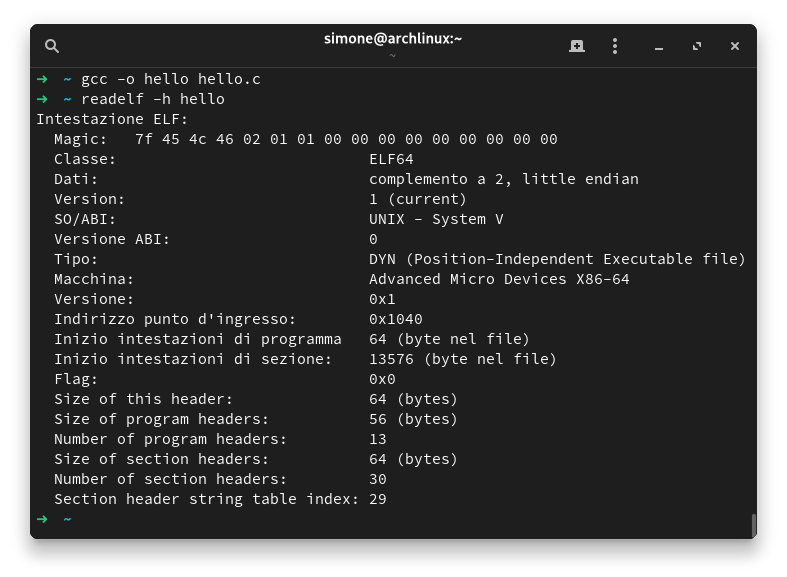
\includegraphics[width=0.6\textwidth]{assets/elf_header.png}
    \caption{Header di un file ELF, letto con readelf}
    \label{fig:elf_header}
\end{figure}

Ma al suo interno troviamo anche le sezioni, tra cui le più rilevanti, con le possibili misure di sicurezza che se mancano potrebbero essere un indicatore che dovrebbe essere portato all'attenzione: \cite{forensic_friday_execs}
\begin{itemize}
    \item \texttt{.text} contiene il codice principale del programma, e rappresenta il focus principale di ogni analisi sul file binario; ha il tipo \texttt{SHT\_PROGBITS} affinché sia eseguibile ma non scrivibile, protezione assolutamente voluta in un programma standard
    \item \texttt{.data} e \texttt{.rodata} contengono i dati del programma, come le variabili o le costanti, a seconda che sia una sezione scrivibile o meno - ad esempio, rilevare un valore di entropia molto alta in questa sezione può essere indice di uso di compressione o crittografia, e va valutato caso per caso se è un comportamento che ci aspettavamo o può essere indicatore di qualcosa di malevolo, proprio per la sua volontà di rendere sempre più difficile l'analisi senza una esecuzione del programma stesso
    \item \texttt{.init} e \texttt{.fini} contengono le procedure di inizializzazione e finalizzazione da eseguire prima del main o prima della terminazione del processo a seguito della fine del normale flusso di esecuzione
\end{itemize}

\begin{figure}[!htb]
    \centering
    \begin{subfigure}[t]{0.48\textwidth}
        \centering
        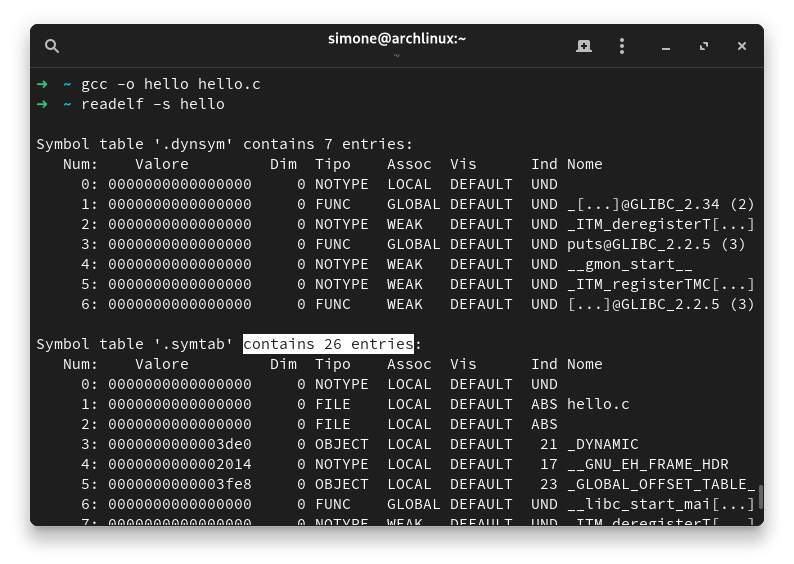
\includegraphics[width=\textwidth]{assets/elf_symtab_full.png}
        \caption{Symbol table originale}
    \end{subfigure}
    \begin{subfigure}[t]{0.48\textwidth}
        \centering
        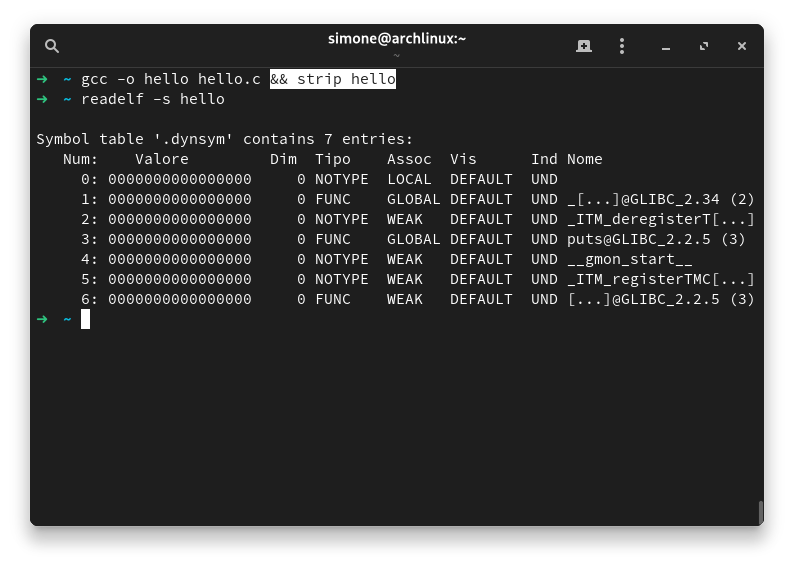
\includegraphics[width=\textwidth]{assets/elf_symtab_stripped.png}
        \caption{Symbol table dopo strip}
    \end{subfigure}
    \caption{Confronto delle symbol table prima e dopo lo strip}
    \label{fig:elf_symtab}
\end{figure}


\subsection{PE}
PE sta per \textbf{Portable Executable} ed è il formato usato nei sistemi Microsoft, derivato dal formato \emph{COFF} di Unix, motivo per cui è spesso identificato come PE/COFF. \cite{forensic_friday_execs}

Viene usato per vari tipi di file, tra cui eseguibili, DLL (Dynamic Link Libraries) e object file.

Anch'esso ha il proprio magic number ai fini di essere identificato correttamente, ed è composto da più header, dove possiamo notare tutta la sua evoluzione come formato. Inizialmente troviamo header specifici di MS-DOS, e successivamente header più caratteristici delle nuove versioni dei PE, includendo sia informazioni di base comuni agli ELF, come il numero di sezioni, di simboli e l'architettura, ma anche la firma digitale dell'immagine del programma per proteggersi da tampering e verificare che l'eseguibile sia realmente proveniente dalla corretta azienda, a meno di leak delle chiavi privati usate per la firma stessa.
\footnote{Maggiori dettagli sono disponibili alla pagina \url{https://learn.microsoft.com/en-us/windows/win32/debug/pe-format}}

\section{Capa: capabilities}
Per i test che vedremo in questa sezione, sono stati scaricati \textbf{40 sample} di malware reali da VirusTotal casualmente, e nelle varie fasi di miglioramento ed evoluzione, soprattutto in merito all'analisi delle capabilities, sono stati fatte numerose prove usando come campioni proprio questi sample.

Per \emph{capabilities} intendiamo le funzionalità che va a usare il programma, ossia ciò che è capace di svolgere durante la propria esecuzione. Esempi di capabilities possono essere la connessione a un server remoto, la modifica di chiavi di registro, o la creazione di un processo figlio, solo per citarne qualcuna.

\begin{figure}[!htb]
    \centering
    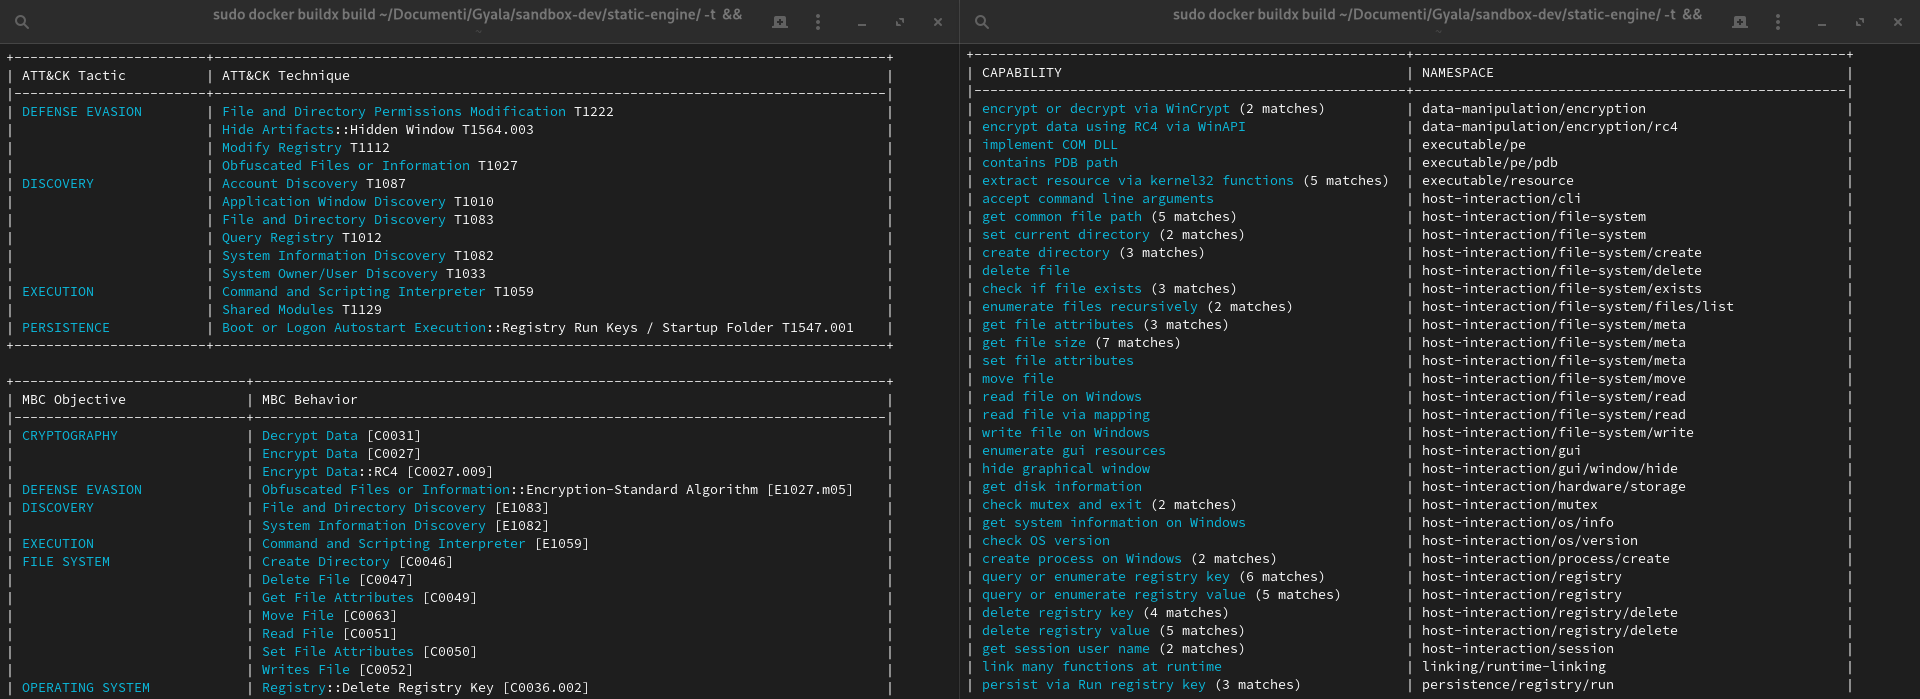
\includegraphics[width=\textwidth]{assets/capa_example_invocation.png}
    \caption{Esempio di esecuzione di capa su pafish64}
    \label{fig:capa_example_invocation}
\end{figure}

Questa estrazione infatti sfrutta lo strumento \textbf{capa},
\footnote{\url{https://github.com/mandiant/capa}}
visto in figura \ref{fig:capa_example_invocation},
tool open-source creato da Mandiant, una delle aziende leader del settore e ora parte di Google,
che permette di andare ad individuare delle capabilities all'interno di un file eseguibile
sfruttando delle regole aventi un proprio formato.
Funziona andando prima ad estrarre delle \emph{features} come le stringhe incluse, codice disassemblato, control flow o file importati.
Poi vengono lanciate le regole su queste features al fine di trarne un'implicazione logica e ottenere informazioni valide a fronte di un match con una o più regole capa.

Il processo di feature extraction si basa in gran parte sull'header che abbiamo appena menzionato nella sezione \ref{chap:static_analysis_binary_structure}, comprese informazioni sulle funzioni esportate, tabella dei simboli (SymTab) e sezioni. Inoltre, il processo di disassemblaggio è molto complesso perché punta sia ad individuare features quali API calls, istruzioni speciali o riferimenti di stringhe/numeri poste in altre sezioni dell'eseguibile (come \texttt{.rodata} per le costanti), ma anche a ricostruire il control-flow minimizzando falsi positivi in caso di dead code o per distinguere tra funzioni e altri \emph{scope}. Alla base di questo step, c'è \texttt{ViviSect Feature Extractor}. \cite{capa_mandiant_blogpost}

Una volta ottenute tutte le features di interesse, si procede a fare il match con le regole.
Una regola capa è una combinazione logica strutturata di match di varie features più di basso livello, per giungere alla conclusione di presenza o assenza di una determinata capability all'interno del software in analisi, espresse sotto forma di file \texttt{YAML}.

Nelle regole, può venir inoltre specificata la tecnica e quindi la tattica, secondo il MITRE ATT\&CK Framework (sez. \ref{chap:mitre_attack}), come visibile nell'output del comando (fig. \ref{fig:capa_example_invocation}).
Questa rappresenta un grande vantaggio per l'integrazione con altri strumenti di Threat Intelligence, per le stesse ragioni favorevoli dell'adozione del framework.

\begin{figure}[!htb]
    \centering
    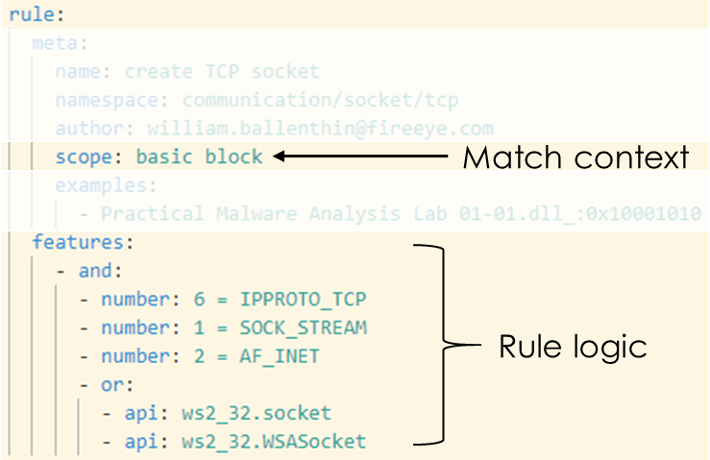
\includegraphics[width=0.6\textwidth]{assets/capa_example_rule.png}
    \caption{Regola capa per rilevare la creazione di un socket TCP}
    \label{fig:enter-label}
\end{figure}

Tuttavia, non tutti gli eseguibili sono supportati da capa, proprio per i motivi precedentemente elencati riguardanti i file offuscati o pacchettizzati. A questo scopo, sono presenti all'interno del set standard di capa, delle regole
(sotto il namespace \texttt{internal/limitation/file} \footnote{\url{https://github.com/mandiant/capa-rules/tree/master/internal/limitation/file}})
che se hanno un match col file in analisi, capa si arresterà non ritenendo più affidabili i propri risultati.
Questo, come vedremo nel prossimo paragrafo, ci costerà troppo tempo e andrà risolto in un altro modo, individuato in \ref{chap:static_analysis_obfuscated}.

\subsection{Analisi dell'uso delle risorse}
Vogliamo analizzare l'uso di risorse da parte di capa con una varietà di file diversi, ossia i 40 sample precedentemente citati da VirusTotal, in termini di spazio e tempo, provando a cercare delle correlazioni con altri dati a nostra disposizione, al fine di eventualmente poter eseguire delle ottimizzazioni.

Bisogna ricordare infatti che il ben più ampio sistema con cui questo progetto si andrà in futuro a interfacciare lavora diverse migliaia di sample ogni mese, per cui è fondamentale ridurre gli sprechi.

All'interno di una macchina virtuale, è stato installato il tool \texttt{capa} insieme ai sample da mettere sotto esame.
Prima di fare ogni tipo di studio, abbiamo bisogno di estrarre dei dati, ottenibili con uno script Python che legge lo stderr del comando, nonché il suo tempo di esecuzione.

Uno dei dati più significativi è il numero di funzioni o blocchi che devono essere analizzate dal feature extractor.
Usando matplotlib, andiamo a validare questa supposizione o confutarla, visualizzando i due elementi in un grafico (fig. \ref{fig:capa_correlation_plot}).

\begin{figure}[!htb]
    \centering
    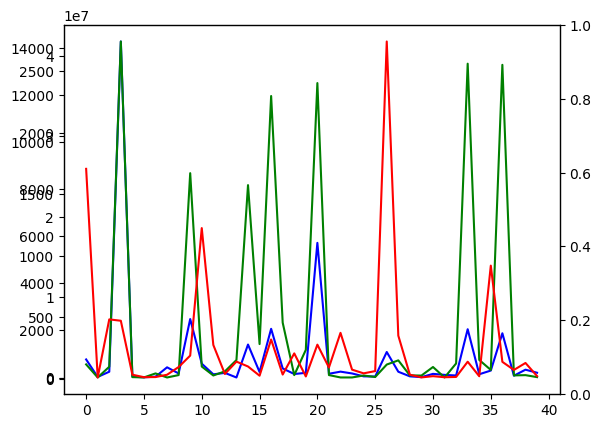
\includegraphics[width=0.6\textwidth]{assets/capa_correlation_plot.png}
    \caption{Correlazione tra tempo di esecuzione (blu) e numero di funzioni/blocchi (verde), assenza di relazione con la dimensione del file (rosso)}
    \label{fig:capa_correlation_plot}
\end{figure}

Siccome su questa metrica non possiamo intervenire in alcun modo, focalizziamoci sull'evitare l'esecuzione di analisi su file che non sono supportati.

%%%%%%%%%%%%%%%%%%%%%%%%%%%%%%%%%%%%%%%%%%%%%%%%%%%%%%%%%%%%%%%%%%%%%%%%%%%%%%%

\subsection{File offuscati}
\label{chap:static_analysis_obfuscated}
Per prima cosa è stato notato come il tool restituisse un diverso \emph{exit code} in base alla corretta esecuzione della feature extraction o meno (listing \ref{code:capa_exit_code}). Da ciò, possiamo rilevare quando un file poteva essere scartato a monte o l'esecuzione di capa ha portato a risultati utili per cui le risorse sono state ben spese.

\begin{code}
\caption{Distinzione tra gli exit code di capa}
\begin{minted}{bash}
function test_file_with_capa() {
    capa "$1" 2>&1 | grep "WARNING:capa: Identified via"
    echo "Exit code (capa): ${PIPESTATUS[0]}"
}

$ test_file_with_capa ./executables/visual_basic_file.exe
WARNING:capa: Identified via rule: (internal) Visual Basic file limitation
Exit code (capa): 14

$ test_file_with_capa ./executables/standard_pe.exe
Exit code (capa): 0
\end{minted}
\label{code:capa_exit_code}
\end{code}

Da qui, abbiamo potuto categorizzare i vari sample in gruppi sulla base del tipo di file, che sia standard (\texttt{pe}) o non supportato da capa (\texttt{packed}, \texttt{installer}, ...).
Creiamo quindi uno script Python che sia in grado di automatizzare questa azione, sia sulla base dell'exit code che dell'output sullo stderr. Otteniamo un JSON come il seguente (estratto per sintesi):

\begin{minted}[samepage]{json}
{
  "./b9c32debb4.exe": "installer",
  "./9f79ea539a.exe": "pe",
  "./4726c42b25.exe": "visualbasic",
  "./e49c42d0b1.exe": "pe",
  .....
}
\end{minted}

La distribuzione della tipologia dei file è riassumibile più graficamente nella figura \ref{fig:capa_file_type_split}, dove notiamo come circa la metà dei sample è difficilmente analizzabile con capa per difetti congeniti dell'analisi statica.
Siccome non possiamo agire direttamente su questo aspetto per eseguire il tool, il prossimo passo sta nel quantificare lo spreco di risorse che si verifica analizzando le capabilities di file che poi porteranno a un fallimento del processo, e se può essere conveniente a livello di trade-off costruire una soluzione per salvaguardare l'uso di risorse saltando del tutto la sua esecuzione (codice \ref{code:static_analysis_capa_count_wasted_time}).

\begin{figure}[!htb]
    \centering
    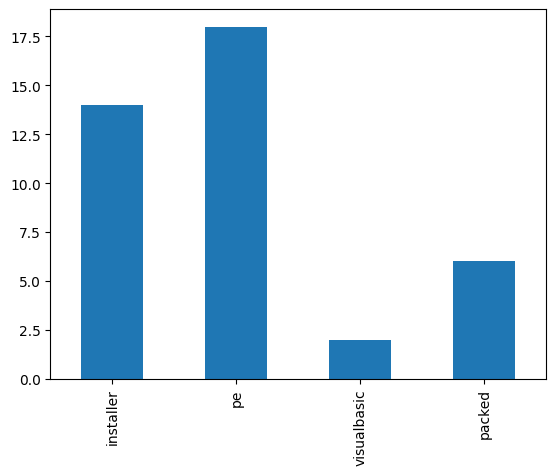
\includegraphics[height=1.8in]{assets/capa_file_type_split.png}
    \caption{Divisione dei sample per tipologia}
    \label{fig:capa_file_type_split}
\end{figure}

\begin{code}
\caption{Calcolo del tempo sprecato eseguendo capa su file non supportati}
\begin{minted}{python}
times = {
    k: v['elapsed_time']
    for k, v in times.items() if file_types[k] != 'pe'
}
avg_wasted_time = sum(times.values()) / len(times)
print(f'{avg_wasted_time:.2f} sec. per unsupported file (avg)')
# 58.77 sec. per unsupported file (avg)
\end{minted}
\label{code:static_analysis_capa_count_wasted_time}
\end{code}

Notiamo che ci mette \textbf{un'eccessiva quantità di tempo} per
eseguire il match delle regole le quali indicano a capa l'impossibilità a proseguire con una soddisfacente confidence, con una media di quasi \emph{un minuto per file}, che moltiplicato su tanti file diventa una grande quantità di tempo totale che potrebbe essere usato in maniera migliore.

\medskip

Ci basta avere i dati di ciò che stiamo trattando, ad esempio l'output desiderato in questo caso sarà del tipo:
\begin{minted}[samepage]{json}
{
    "capa": {
        "format": "packed",
        "arch": "i386",
        "os": "windows"
    }
}
\end{minted}

Come soluzione, dobbiamo trovare un sistema per riconoscere preventivamente che si tratti di un file che non è possibile analizzare con capa.

%\newpage
\section{Riconoscitore custom del tipo di file}
Partendo dalla necessità di velocizzare l'operazione di riconoscimento del file, in sostituzione dell'esecuzione del comando \texttt{capa -r anti-analysis} che può portare a richiedere diversi minuti a seconda del numero di funzioni presenti nel file, come visto in figura \ref{fig:capa_correlation_plot},
dobbiamo ricorrere a una diversa soluzione.

Dato che si tratta di un problema di enumerazione, non aveva senso andare a creare e mantenere un proprio riconoscitore di ogni possibile formato di un file. Ad esempio, già solo per quanto riguarda i file pacchettizzati, esistono tantissimi packer e tanti ne esisteranno in futuro.

Inoltre, spesso malware usano packer personalizzati, che hanno leggere differenze da quelli noti e si correrebbe il rischio di creare uno strumento poco efficace.
Per questi e altri motivi quali il tempo a disposizione, si era inizialmente scelto di usare come base uno strumento noto (\texttt{Detect-It-Easy}) per fare una prima analisi, affiancato da uno script Python custom che decide quali operazioni svolgere a seconda del tipo di file, va a fare il parsing del JSON dato in output e si integra nello script Bash creando un layer di astrazione col resto del workflow.
Infatti, nel caso servisse modificare lo strumento sottostante, sarebbe sufficiente adattare la traduzione dall'output specifico del tool al contratto stabilito col resto del programma per rendere seamless questa variazione, anche sostanziale.
Tuttavia, ci sono alcuni tipi che anche Detect-It-Easy fallisce a riconoscere, portando poi a un crash di capa quando eseguito.

Per questo motivo è stato creato un \textbf{custom detector}, scritto in Python, che implementa in maniera molto più efficiente e diretta, le sole regole di capa che riconoscono i file specifici su cui non è in grado di lavorare.

Di seguito possiamo osservare come funziona per dei tipi famosi di questi strumenti, ovvero il packer UPX e l'installer InnoSetup.
Sono state usate caratteristiche e regole note
\footnote{\url{https://github.com/mandiant/capa-rules/tree/e88db21de4d4cf9f7abec9177fab11240075036b/anti-analysis/packer}}
per eseguire la detection.

La lettura degli header del file PE sfrutta la libreria Python \texttt{pefile} per non eseguire l'intero parsing a mano dei byte degli header e non essere dipendenti da implementazioni native dell'OS come con l'uso dell'header \texttt{<windows.h>} in un programma C.

\begin{figure}[!htb]
    \centering
    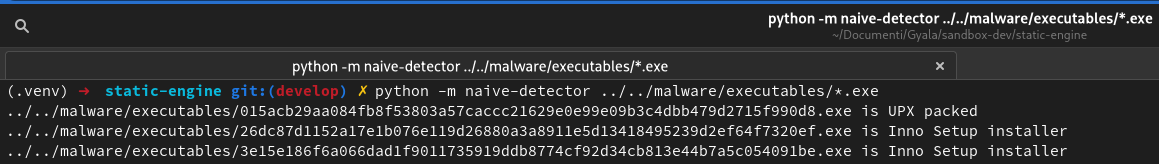
\includegraphics[width=\textwidth]{assets/custom_file_detector_output.png}
    \caption{Custom file detector output}
\end{figure}

\subsection{UPX}
Le regole più comuni
\footnote{\url{https://github.com/mandiant/capa-rules/blob/e88db21de4d4cf9f7abec9177fab11240075036b/anti-analysis/packer/upx/packed-with-upx.yml}}
per riconoscere UPX impongono di leggere le sezioni, e vedere se queste contengono \texttt{UPX0} o \texttt{UPX1}.

Facciamo una comparazione tra la regola capa per il rilevamento e il codice del riconoscitore.

\noindent\begin{minipage}{.35\textwidth}
       \begin{minted}{yaml}
features:
    - format: pe
    - or:
      - section: UPX0
      - section: UPX1
       \end{minted}
\end{minipage}
\begin{minipage}{.4\textwidth}
       \begin{minted}{python}
def is_upx(file_path):
    file_sections = get_section_names(file_path)
    upx_sections = [ "UPX0", "UPX1" ]
    for upx_section in upx_sections:
        if upx_section in file_sections:
            return True
    return False
       \end{minted}
\end{minipage}

\bigskip

Andando però a sfruttare la libreria Python per il parsing del file PE senza ricorrere a implementazioni native Windows:

\begin{minted}{python}
import pefile

def get_section_names(file_path):
    pe = pefile.PE(file_path)
    sections_set = {
        section.Name.decode().strip().strip('\x00')
        for section in pe.sections
    }
    pe.close()
    return sections_set
\end{minted}

\subsubsection{Analisi preliminare con readelf}
Notiamo come questa tecnica funzioni solo in ambito Windows, mentre su sistemi GNU/Linux notiamo con strumenti quali \texttt{readelf} che il file sia privo di header delle sezioni
(in accordo con la regola CAPA stessa, che infatti include questo match solo se ci troviamo su un file PE, come indicato dall'apposita riga \texttt{- format: pe}).

Negli eseguibili in formato ELF infatti è più comune trovare una situazione in cui l'header delle sezioni è mancante. Infatti, tale informazione non è usata in alcun modo dal kernel durante il caricamento in memoria del programma, nella creazione della process image. Inoltre, non è indicatore di azioni malevoli, ma sicuramente della volontà di rendere l'analisi più difficile, il cui caso può riguardare anche binari di produzione di software proprietario closed-source.

\subsubsection{Analisi dell'entropia}
Una caratteristica comune di binari compressi o con payload criptati è l'aumento di entropia. Infatti, sia la compressione che la crittografia vanno ad aumentare l'entropia all'interno di uno stesso blocco di file, motivo per cui è essenziale eseguire la compressione di un file prima della sua crittazione, altrimenti l'algoritmo di compressione sarebbe molto meno efficace.

Come esempio, è stato preso un eseguibile il cui sorgente è ininfluente, compilato con il compilatore C \texttt{gcc} e poi calcolata l'entropia sia prima che dopo averlo pacchettizzato con UPX. I grafici sono stati generati tramite l'ausilio di uno script Python creato ad-hoc e sfruttando il calcolo dell'entropia di Shanon.

\begin{figure}[htbp]
    \centering
    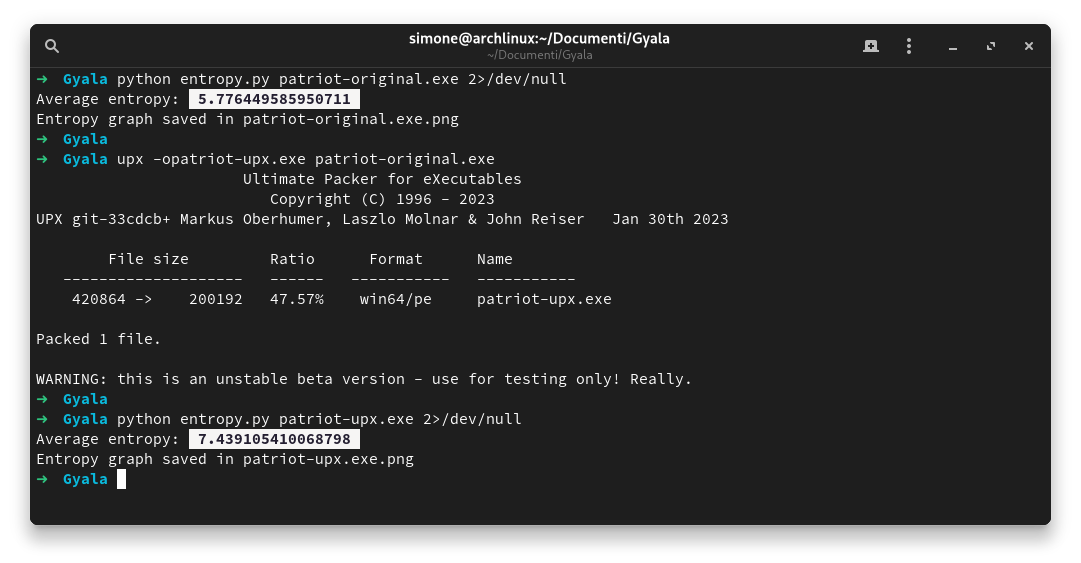
\includegraphics[width=0.75\textwidth]{assets/entropy_script_terminal.png}
    \caption{Esecuzione dello script per il calcolo dell'entropia e uso di UPX}
    \label{fig:entropy_script_terminal}
\end{figure}

\begin{figure}[!htb]
    \centering
    \begin{subfigure}[t]{0.48\textwidth}
        \centering
        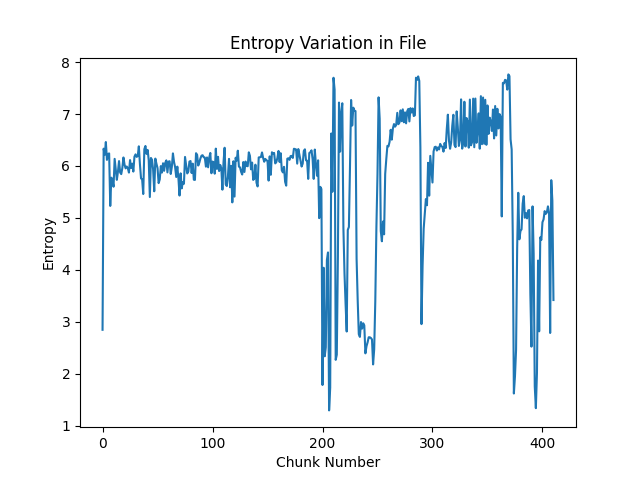
\includegraphics[width=\textwidth]{assets/patriot-original.exe.png}
        \caption{Entropia del file originale}
    \end{subfigure}
    \begin{subfigure}[t]{0.48\textwidth}
        \centering
        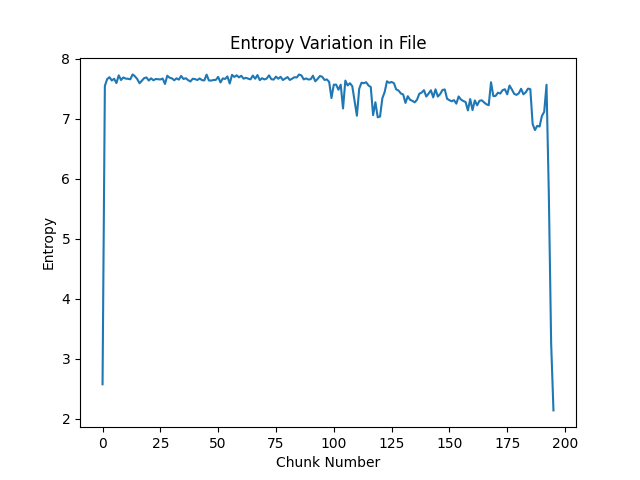
\includegraphics[width=\textwidth]{assets/patriot-upx.exe.png}
        \caption{Entropia del file pacchettizzato con UPX}
    \end{subfigure}
    \caption{Confronto dell'entropia prima e dopo l'uso di UPX}
    \label{fig:entropy_upx_comparison}
\end{figure}

\begin{figure}[htbp]
    \begin{subfigure}[t]{0,48\textwidth}
        \begin{gather*}
            H(x) = - \sum_{i=1}^{n} \frac{count_i}{N} \log{\left(\frac{count_i}{N}\right)}
        \end{gather*}
    \end{subfigure}
    \begin{subfigure}[t]{0,48\textwidth}
        \begin{minted}{python}
def calculate_entropy(data):
    entropy, size = 0, len(data)
    if size <= 1: return entropy

    byte_count = [0] * 256
    for byte in data:
        byte_count[byte] += 1

    for count in byte_count:
        if count > 0:
            probability = float(count) / size
            entropy -= probability \
                * math.log(probability, 2)

    return entropy
        \end{minted}
    \end{subfigure}
    \caption{Formula dell'entropia di Shannon e codice Python per il calcolo su un chunk}
    \label{fig:shannon_entropy_formula}
\end{figure}

%%%%%%%%%%%%% http://blog.dkbza.org/2007/05/scanning-data-for-entropy-anomalies.html
%%%%%%%%%%%%% https://fsec404.github.io/blog/Shanon-entropy/

\subsection{Inno-Setup Installer}
Con Inno-Setup, possiamo notare come sia ancora più semplice il riconoscimento. Infatti, non abbiamo bisogno di andare a vedere le sezioni, ma è sufficiente controllare la presenza di alcune stringhe statiche nel file.

Nuovamente, andiamo a paragonare la regola capa alla nostra implementazione:

\begin{minted}{yaml}
features:
    - and:
      - string: /^Inno Setup Setup Data \(/
      - string: /^Inno Setup Messages \(/
\end{minted}

\begin{minted}{python}
def is_innosetup(file_path):
    BUFFER_SIZE = 65536
    with open(file_path, 'br') as f:
        match_setup, match_messages = False, False
        buffer = f.read(BUFFER_SIZE)
        overlap = len(b'Inno Setup Setup Data (')

        while len(buffer) > overlap and (not match_setup or not match_messages):
            # Match inside current buffer
            if not match_setup and b'Inno Setup Setup Data (' in buffer:
                match_setup = True
            if not match_messages and b'Inno Setup Messages (' in buffer:
                match_messages = True
            
            # Read next buffer, allowing for overlap
            buffer = buffer[-overlap:] + f.read(BUFFER_SIZE)
    
    return match_setup and match_messages
\end{minted}

\subsection{Design scalabile e modulare}
Si nota immediatamente come una tale implementazione è poco scalabile e presenta numerose ridondanze da rimuovere.

Studiando le regole di interesse all'interno del repository GitHub \textit{capa-rules}, osserviamo come le regole siano principalmente di due categorie: basate su match di stringhe o basate su match di nomi di sezioni nel file eseguibile.

Da questa osservazione, elaboriamo la struttura del programma software di detection. Precisamente, decidiamo di strutturarlo in classi dove ogni regola è una classe a sé, e individuiamo le seguenti classi padre (figura \ref{fig:base_custom_static_analyzer_uml}):
\begin{itemize}
    \item \texttt{BaseRule} conterrà le logiche di base che possiede una regola, tra cui un getter per il nome e un metodo \texttt{match()}
    \item \texttt{StringRule} conterrà il codice unico per tutte le regole che basano il loro match sulla presenza di determinate stringhe all'interno del file, quindi la classe figlia dovrà solo fornire le stringhe da cercare e la logica di match (ad esempio: tutte le stringhe richieste devono essere state trovate = and logico; una sola stringa trovata è sufficiente = or logico)
    \item \texttt{SectionRule} analogamente a prima conterrà le procedure di estrazione delle sezioni dal file, con la logica di match nelle classi figlie, ossia le effettive regole.
\end{itemize}

Sempre al fine di ottimizzare i tempi di esecuzione di questo rilevamento statico sul file eseguibile,
andiamo a creare una classe wrapper sopra \texttt{pathlib.Path} che esporrà i metodi per leggere le sezioni, procedura lenta se ripetuta per ogni singola regola, e alcune altre funzioni di utilità come la rilevazione del tipo basilare di file (PE o ELF) eseguibile tramite l'ausilio di \texttt{libmagic}, la stessa che permette al comando \texttt{file} di operare.
Quindi da un lato è stata aumentata l'astrazione tra la business logic del programma e i dettagli implementativi delle librerie sottostanti, dall'altro possiamo aggiungere meccanismi di lazy-loading e caching di tali informazioni richieste.

\begin{figure}[H]
    \centering
    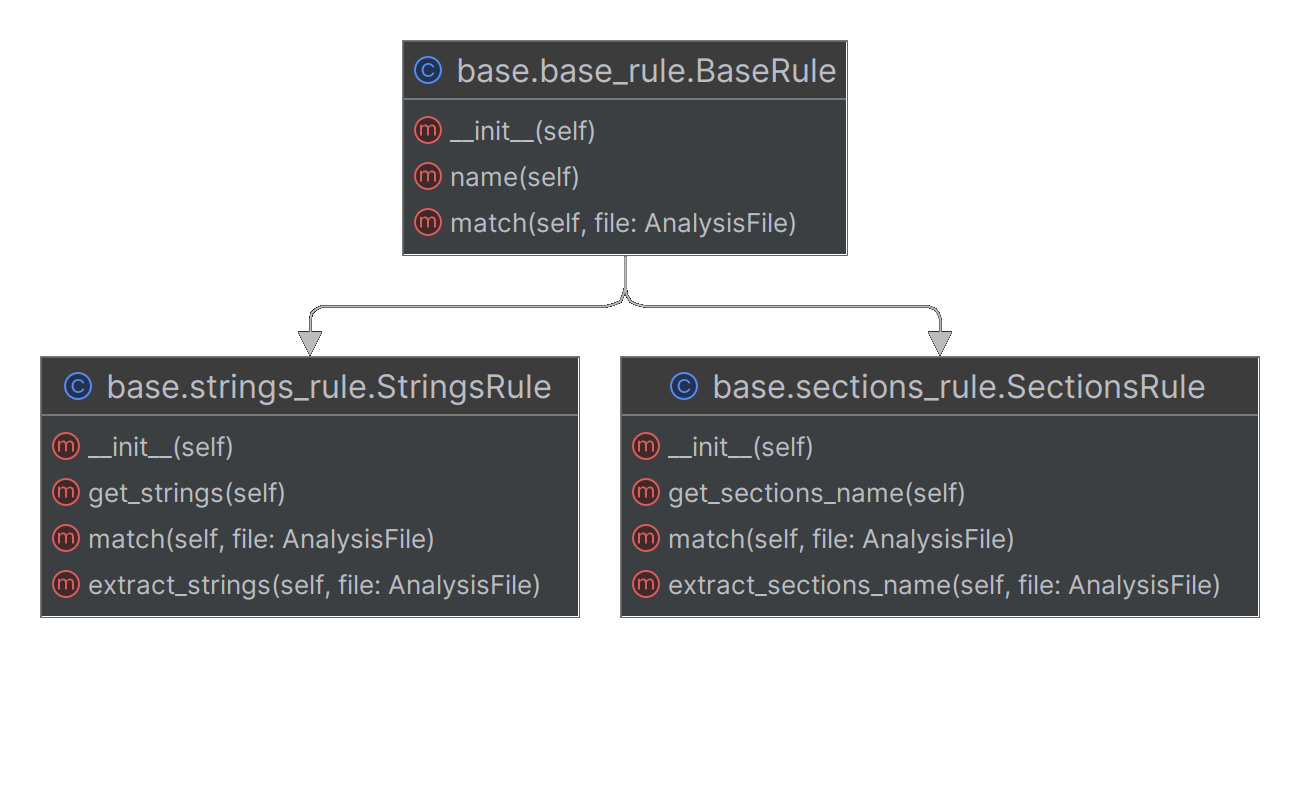
\includegraphics[width = 0.8\textwidth]{assets/base_custom_static_analyzer.png}
    \caption{Diagramma UML delle classi}
    \label{fig:base_custom_static_analyzer_uml}
\end{figure}

\begin{code}
    \begin{minted}[samepage]{python}
class InnoSetupDetector(StringsRule):
    def name(self) -> str:
        return 'executable/installer/inno-setup'

    def get_strings(self) -> list[bytes]:
        return [
            b'Inno Setup Setup Data (',
            b'Inno Setup Messages (',
        ]

    def match(self, file: AnalysisFile) -> bool:
        # && logic
        return len(self.extract_strings(file)) == len(self.strings)
    \end{minted}
    \caption{Regola di riconoscimento di InnoSetup, usando la nuova architettura}
    \label{code:enter-label}
\end{code}

\section{Yara: signature-based}
Sia per statici che in memoria dei processi.

Ora però usate solo per analizzare staticamente un file eseguibile.

\section{FLARE Floss}
Teoria: \url{https://github.com/mandiant/flare-floss/blob/master/doc/theory.md}

\section{Automazione su AWS}

\subsection{Scrittura dei parser}
Parser per capa e yara.

Parser dal file testuale, con schemini.

\subsection{Architettura serverless}
L'architettura è ben riassunta nel seguente diagramma, che andremo a spiegare:
\begin{figure}[htbp]
    \centering
    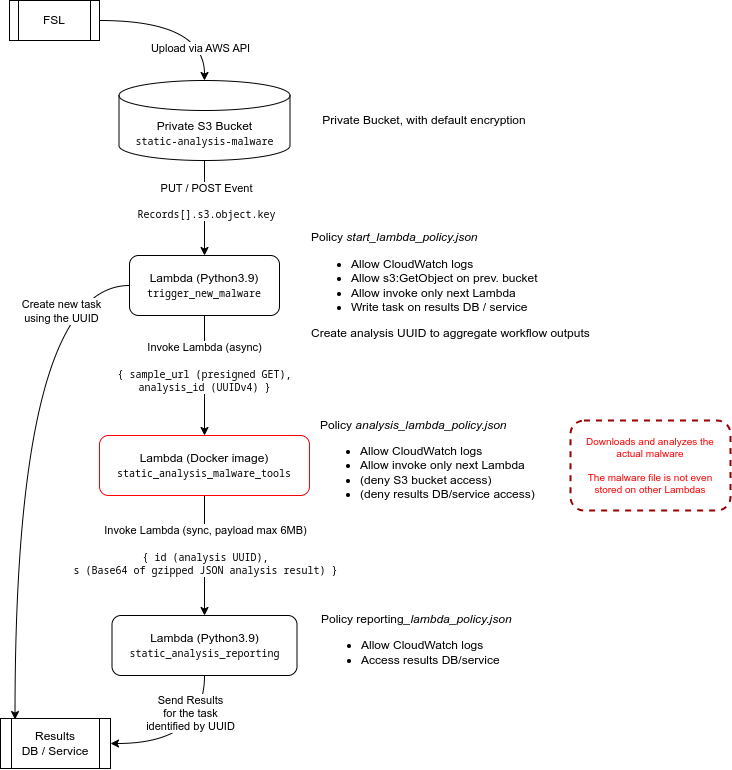
\includegraphics[width=\textwidth]{assets/aws_static_lambdas_architecture.png}
    \caption{Archittetura su AWS con i vari componenti coinvolti}
    \label{fig:aws_static_lambdas_architecture}
\end{figure}

\begin{figure}[htbp]
    \centering
    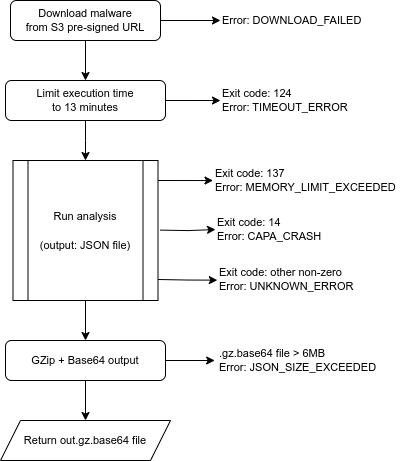
\includegraphics[width=0.75\textwidth]{assets/docker_static_analysis_flow.png}
    \caption{Workflow dell'analisi in \texttt{static\_analysis\_malware\_tools} e possibili errori}
    \label{fig:enter-label}
\end{figure}

\begin{figure}[htbp]
    \centering
    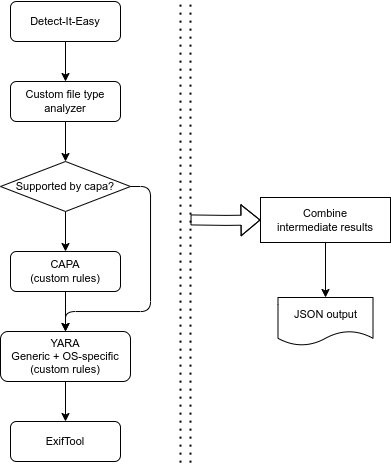
\includegraphics[width=0.75\textwidth]{assets/static_run_analysis_internal_tools.png}
    \caption{Workflow processo interno di \texttt{run\_analysis}}
    \label{fig:enter-label}
\end{figure}

\subsection{Creazione dell'immagine}
Prima era enorme (naive approach), poi ridotta sfruttando il multistage.

\begin{figure}[H]
    \centering
    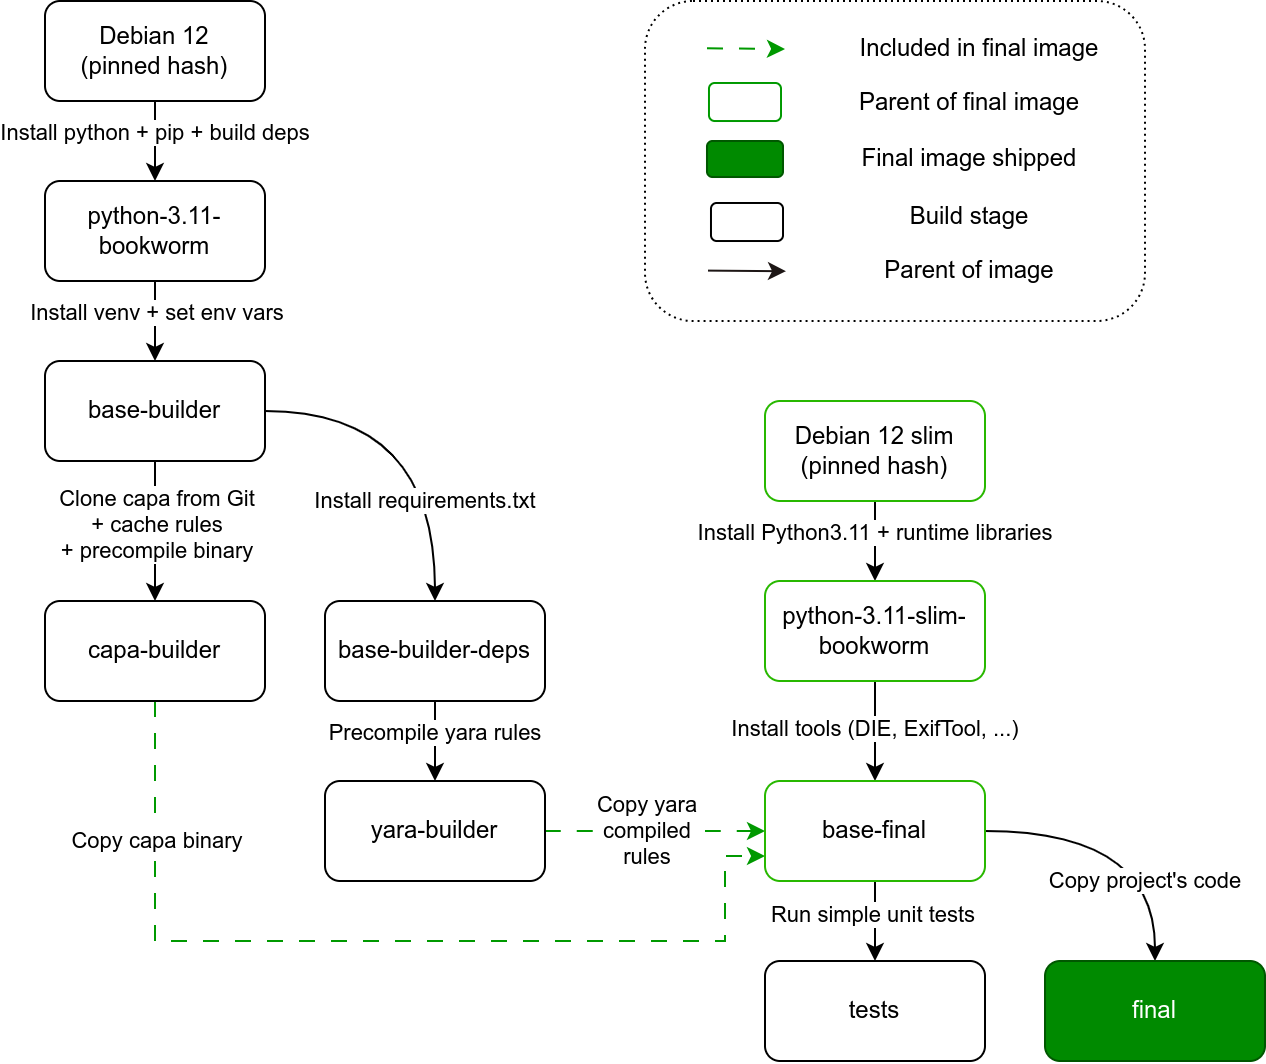
\includegraphics[width=\textwidth]{assets/dockerfile.png}
    \caption{Docker multi-stage build, con le immagini intermedie}
    \label{fig:static_dockerfile_multistage_build}
\end{figure}

Uso di CMD/ENTRYPOINT così da rendere l'immagine usabile sempre, che sia da URL o da cartella su cui itera.


Serve eseguirla su Lambda = serve rispettare la Runtime Interface!


\subsection{Deploy e hardening}
Sicurezza e varie policy (hardening)

\subsection{Limiti delle Lambda}

CPU time e memoria. Gestione degli errori (status 137 OOM).

\begin{figure}[H]
     \begin{subfigure}[b]{0.5\textwidth}
         \centering
         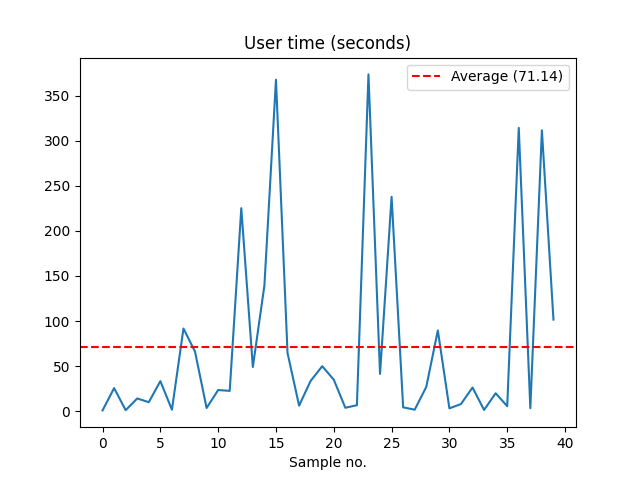
\includegraphics[width=\textwidth]{assets/static_analysis_exec_cpu_time.png}
         \caption{CPU}
         \label{fig:static_analysis_exec_cpu_time}
     \end{subfigure}
     \begin{subfigure}[b]{0.5\textwidth}
         \centering
         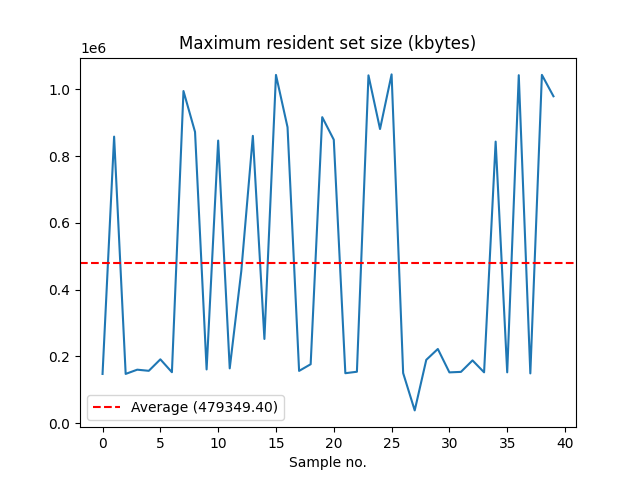
\includegraphics[width=\textwidth]{assets/static_analysis_exec_memory.png}
         \caption{Memoria}
         \label{fig:static_analysis_exec_memory}
     \end{subfigure}
     \label{fig_static_analysis_exec_stats}
     \caption{Uso delle risorse eseguendo analisi statica su malware reali presi a campione}
\end{figure}

6MB / 256KB in base a sync/async invocation.

\begin{figure}[H]
    \centering
    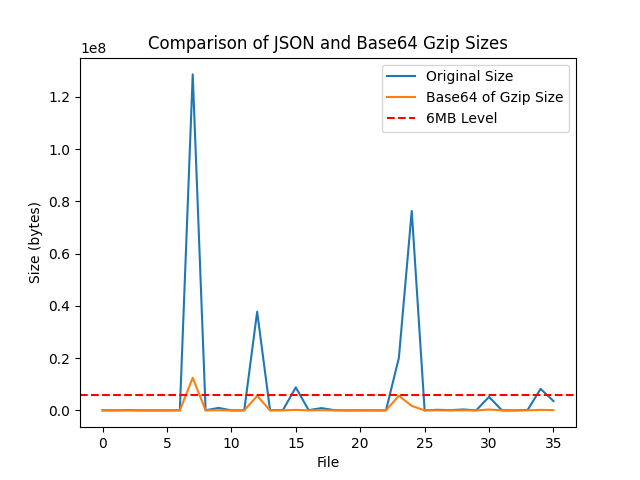
\includegraphics[width=0.6\textwidth]{assets/static_analysis_results_size.png}
    \caption{Dimensione del file di output originale e post-compressione gzip + base64}
    \label{fig:static_analysis_results_size}
\end{figure}

\subsection{Costi del servizio}
Le prossime analisi si baseranno sui seguenti parametri di riferimento forniti sulla base dello storico aziendale e delle aspettative di uso reale del servizio:
\begin{table}[H]
    \centering
    \begin{tabular}{|l|l|}
        \hline
        \textbf{Parametro}             & \textbf{Valore (al mese)}       \\ \hline
        Numero di sample da analizzare & 1.000.000                       \\
        Memoria media richiesta        & 512 MB (limite massimo: 1024MB) \\
        Tempi medio di esecuzione      & 70 secondi                      \\ \hline
    \end{tabular}
\end{table}

Inoltre, si sottolinea come i costi dei servizi AWS subiscano inflessioni nel tempo, per cui questa stima è sufficientemente valida al momento della scrittura di questo documento.

\begin{table}[H]
    \centering
    \begin{tabular}{|l|l|}
        \hline
        \textbf{Servizio}         & \textbf{Costo stimato (al mese)} \\ \hline
        S3 Bucket (standard tier) &                                  \\
        Lambda start              &                                  \\
        Lambda di analisi         &                                  \\
        Lambda di fine rapporto   &                                  \\ \hline
        Costo stimato totale      & € 750,00                         \\ \hline
    \end{tabular}
\end{table}

\section{Versioning}
Per il versioning, è stato creato un repository Git sul server GitLab aziendale.

Per ogni modifica viene creato un commit, come è standard.

Tuttavia, ci sono alcuni aspetti dell'organizzazione che ha senso sottolineare.

\subsection{Branch Naming Convention}
Per la gestione del repository,e in particolare i suoi branch, si seguono rigidamente queste convenzioni:
\begin{itemize}
    \item \texttt{main} è il branch principale dove deve essere presente solo codice finito e considerabile stabile a tutti gli effetti;
    \item \texttt{develop} è dove si tiene il codice che si considera usabile ma non ancora sufficientemente testato o pronto all'uso in produzioni così com'è - su questo branch infine è dove viene fatto il merge dei successivi branch più specifici;
    \item \texttt{feature/<feat-name>} è l'insieme di tutti i branch, originati da \emph{develop}, dove si lavora all'implementazione di una specifica funzione - ciò permette di mantenere il branch \emph{develop} funzionante, privo di funzioni non completamente realizzate, e diminuisce le interferenze tra chi sta lavorando sulla stessa codebase ma su funzioni distinte tra loro - e il prefisso \textbf{feature/} identifica chiaramente che si tratta di un branch dove si lavora solo ed esclusivamente su una sola funzionalità;
    \item \texttt{refactor/<ref-name>} invece rappresenta l'insieme dei branch dove si fa, con diversi gradi di complessità, refactoring del codice - ad esempio, nel progetto è stato realizzato un branch di refactoring per passare dall'uso di \texttt{os.path} al modulo Python \texttt{pathlib} per una maggiore usabilità
\end{itemize}

Infine, per un maggiore controllo, il merge dai branch secondari (\texttt{feature/} e \texttt{refactor}) vengono fatti attraverso l'uso di \emph{Merge Request} (o \emph{Pull Request}, a seconda che si usa la nomenclatura di GitLab o di GitHub).
In questo modo, è possibile interagire sul merge commentando o richiedendo revisioni di co-workers.

Non siamo ancora giunti al punto di rilasciare il progetto e attribuirgli una versione, ma in tal caso è ideale usare convenzioni standard come \emph{Semantic Versioning}, e usare tale stringa come \textbf{tag} sul repository Git.

\begin{figure}[h!]
    \centering
    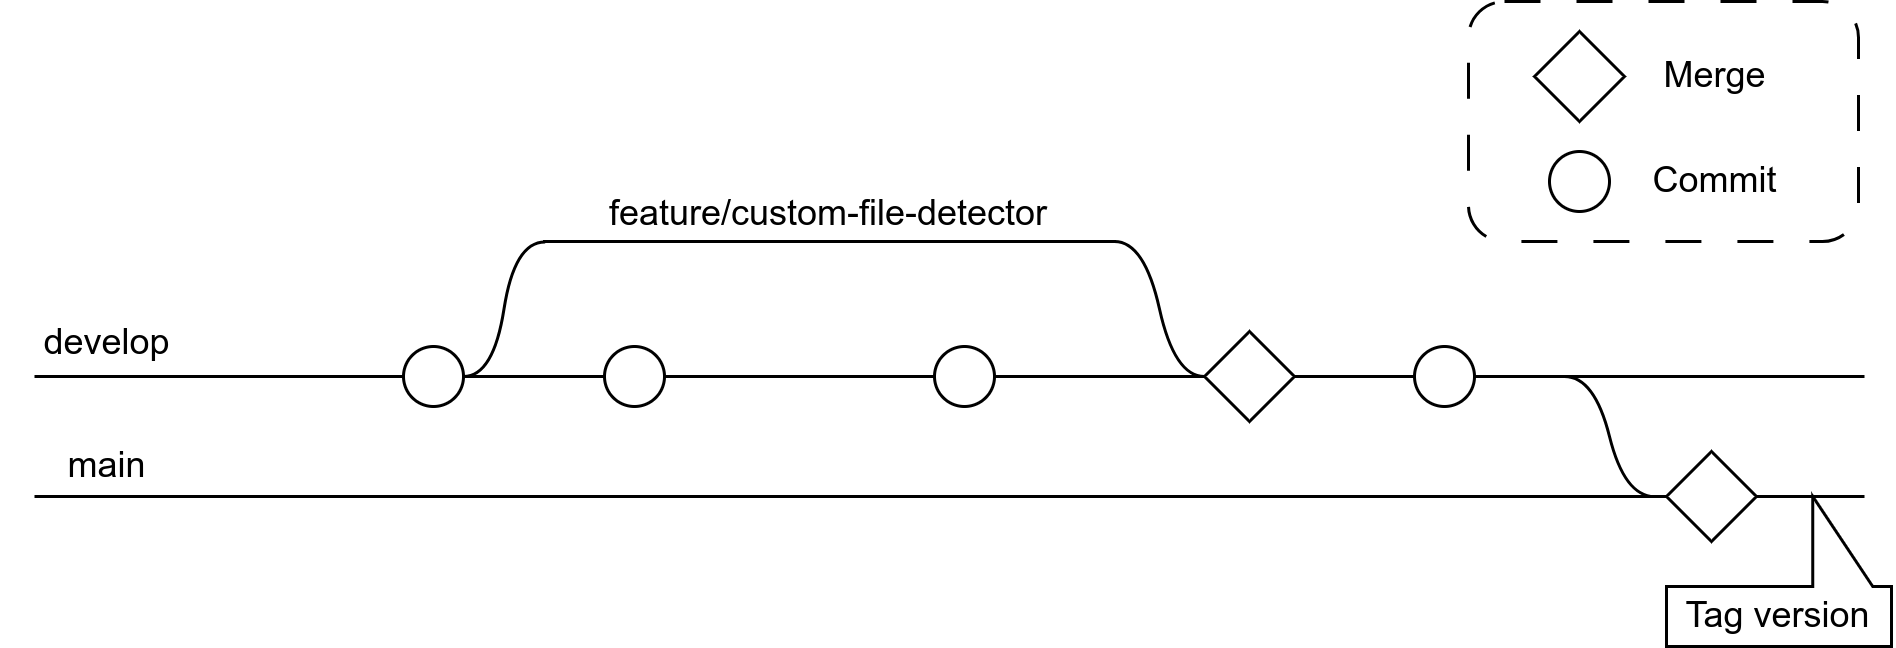
\includegraphics[width=\textwidth]{assets/git_branches_diagram.png}
    \caption{Struttura dei branch Git}
    \label{fig:git_branches_diagram}
\end{figure}